\chapter{Systems Design}

In this chapter, I present the solution for design the Delta robot. 
Mechanical design, as well as it's advantage and disadvantage are described in section 1. Subsequently, Section 2 presents electronic design and solution to anti-interference. In the final section the software design and solution to control the robot are elaborated to conclude this chapter.

\section{Mechanical Design}

The mechanical design of the robot must be simple yet effective. Also, the parts used for the frame and the moving actuator arms needs to be quite cheap. The proportions of the actuator arms are not that crucial as the control system can take the slight proportion errors into account if it is programmed correctly. However, to make the robot as effective as possible, the actuator arm proportions should be designed so that all three of them are identical and that the mechanical design can be designed in a simple way. By default, the mechanical system design should not be my strongest aspect. I'm planning on doing the actuator arms so that they can be adjusted to get the robot to work as effective as possible. The goal is to make our robot lightweight and cheap but be sturdy and rigid enough for the actuator to be  accurate. The actual way to achieve our goals will be achieved through using Acrylic glass(\glspl{pmma}) sheets and parts, whose structural strength will be achieved through effective structural design.

The target screen size that the robot will operation on is $(4" \ast 6")$. With this in mind, the length of the lower arms can be obtained by simulating the arms in GeoGebra\cite{GeoGebra_thesis}(the dynamic mathematics software for education) and then modeling them in SolidWorks. The only guideline I had was to keep the upper arms shorter than the lower arms for the best range and keep the two rods of each lower arm as far apart as possible for stability.
\begin{figure}[H]	
	\centering
	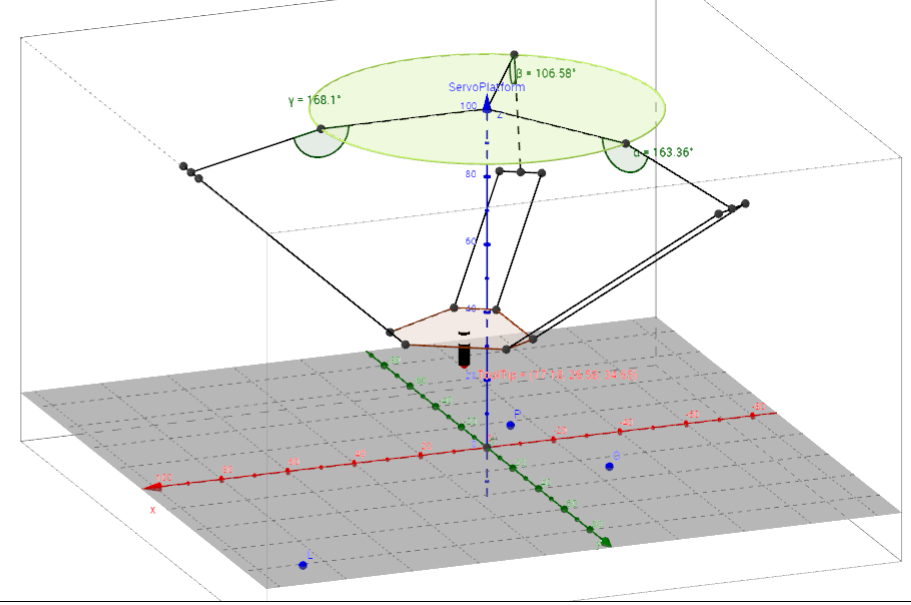
\includegraphics[width=\maxwidth{15cm}, keepaspectratio]{Chapters/Fig/3D_delta_robot_simulator.png}
	\caption{3D Delta Robot simulator\cite{GeoGebra_deltarobot_simulator_thesis}}
	\label{fig:3D_delta_robot_simulator}
\end{figure}

I simulate Delta robot by GeoGebra and find out the parameters needed, show in Table.\ref{tab:key_parameters_of_robot_geometry}. After that, I design the robot's model on SolidWorks.
\begin{figure}[H]
	\centering
	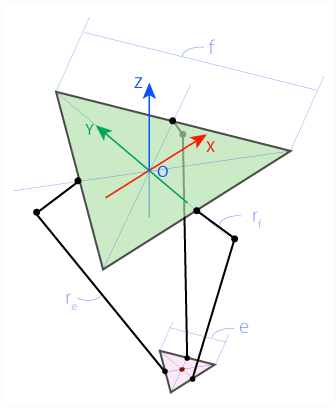
\includegraphics[width=\maxwidth{10cm}, keepaspectratio]{Chapters/Fig/key_parameters.png}
	\caption{Key parameters of robot's geometry}
	\label{fig:key_parameters_value}
\end{figure}

\begin{table}[H]
	\centering
	\caption{Key parameters of robot's geometry}	
	\label{tab:key_parameters_of_robot_geometry}
	\begin{tabularx}{0.65\textwidth}{ll}
		\toprule
		\textbf{Parameter} & \textbf{Length(mm)} 		\\
		\midrule
		Side of the fixed triangle(f) & 352.78 			\\
		\midrule
		Side of the end effector triangle(e) & 96.54 	\\
		\midrule
		Length of the upper joint($r_{f}$) & 69.85 		\\
		\midrule
		Length of the parallelogram joint($r_{e}$) & 306.00 \\
		\bottomrule
	\end{tabularx}
\end{table}
\begin{figure}[H]
	\centering
	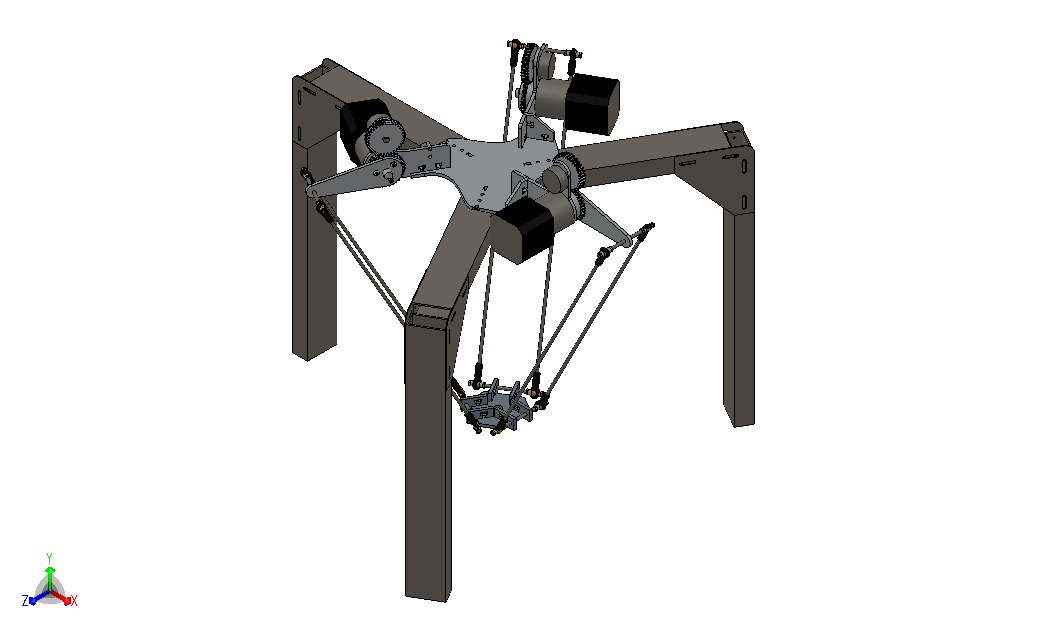
\includegraphics[width=\maxwidth{15cm}, keepaspectratio]{Chapters/Fig/robot_isometric_view.png}
	\caption{Isometric view of Delta robot}
	\label{fig:robot_isometric_view}
\end{figure}

\begin{figure}[H]
	\centering
	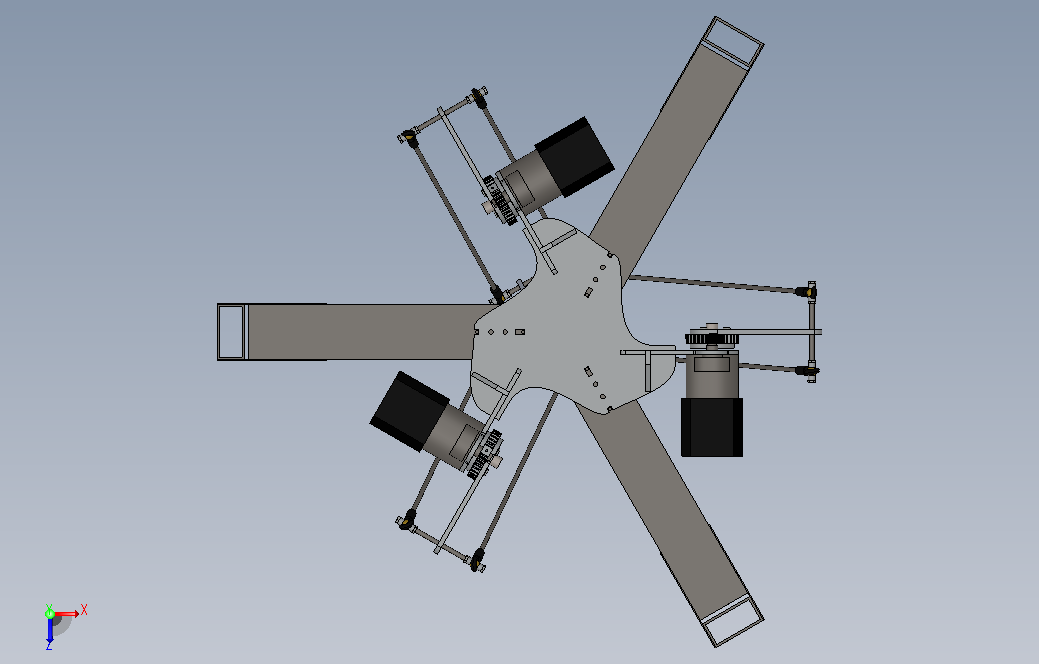
\includegraphics[width=\maxwidth{15cm}, keepaspectratio]{Chapters/Fig/robot_top_view.png}
	\caption{Top view of Delta robot}
	\label{fig:robot_top_view}
\end{figure}

I made the upper-to-lower arm length ratio much smaller in order to get the precision over a larger range on the XY plane, at the expense of Z traversal. If the upper arms were quite long, inrelation with the lower arm, It will move really great range in the Z dimension. But for a phone-testing robot, this is useless. Since the arms were so long, small movements in the motors created large movements in the manipulator. I got poor results in the accuracy of the action. For the best range of motion for touching, when the touch-pen is centered on the phone, the upper arms should stay near in horizontal direction, relative to the robot.
And potentiometers were linked to the output shaft through gears.

\subsubsection{List of parts of Delta robot:}
\begin{itemize}
		\item Custom mechanical parts cut from 3mm thick Acrylic glass(\glspl{pmma})
		\item Three Gear Ratio 5:1 Nema 17 Stepper Motor 0.4A 12V
		\item 2.5m threaded rod $\phi$3mm
		\item A bunch of various M3 socket cap screws and nuts
		\item Traxxas 5347 Rod Ends with Hollow Balls Large Revo\cite{traxxas_5347_thesis}
		\item Arduino 2560 microcontrollers
		\item 3 Pololu A4988 stepper motor driver
		\item 12V power supply
		\item Power filtering capacitor, 1 x 104 (0.1$\mu$F/50V) ceramic capacitor and 1 x Electrolytic capacitor( 2000$\mu$F, 16V)
		\item 3 rotary potentiometer 10K ohms
		\item LCD 16x2
\end{itemize}


\section{Control circuit design}

The electronic design is a rather simple and straight forward step. I'm using an Arduino MEGA 2560 board as our control board and Stepper Motor as motors, which is controlled by Pololu A4988 Driver. To get status of stepper motor, I using 10k ohm potentiometer linked to the output stepper motor's shaft through gears. In addition, LCD 16x2 is used to display the value of potentiometer in real time.

\subsection{Stepper motor controller circuit}

Here are the pinouts from the Pololu A4988 driver and the corresponding pin connection on the Arduino MEGA 2560:
\begin{table}[H]
	\centering
	\caption{The pinouts from the Pololu A4988 driver and the corresponding pin connection on the Arduino MEGA 2560}	
	\label{tab:A4988_connectto_Arduino}
	\begin{tabularx}{0.65\textwidth}{lll}
		\toprule
		\textbf{Driver index} & \textbf{A4988 Pin} & \textbf{Arduino Pin} \\
		\midrule
		\multirow{3}{*}{1st}	& Dir       & 7            \\
		                   	 	& Step      & 6            \\
		                   	 	& Enable    & 5            \\
		\midrule
		\multirow{3}{*}{2nd} 	& Dir       & 4            \\
		                   	 	& Step      & 3            \\
		                   	 	& Enable    & 2            \\
       	\midrule
      	\multirow{3}{*}{3rd} 	& Dir       & 14           \\
		                   	 	& Step      & 15           \\
		                   		& Enable    & 16           \\
		\bottomrule
	\end{tabularx}
\end{table}

\begin{figure}[H]
	\centering
	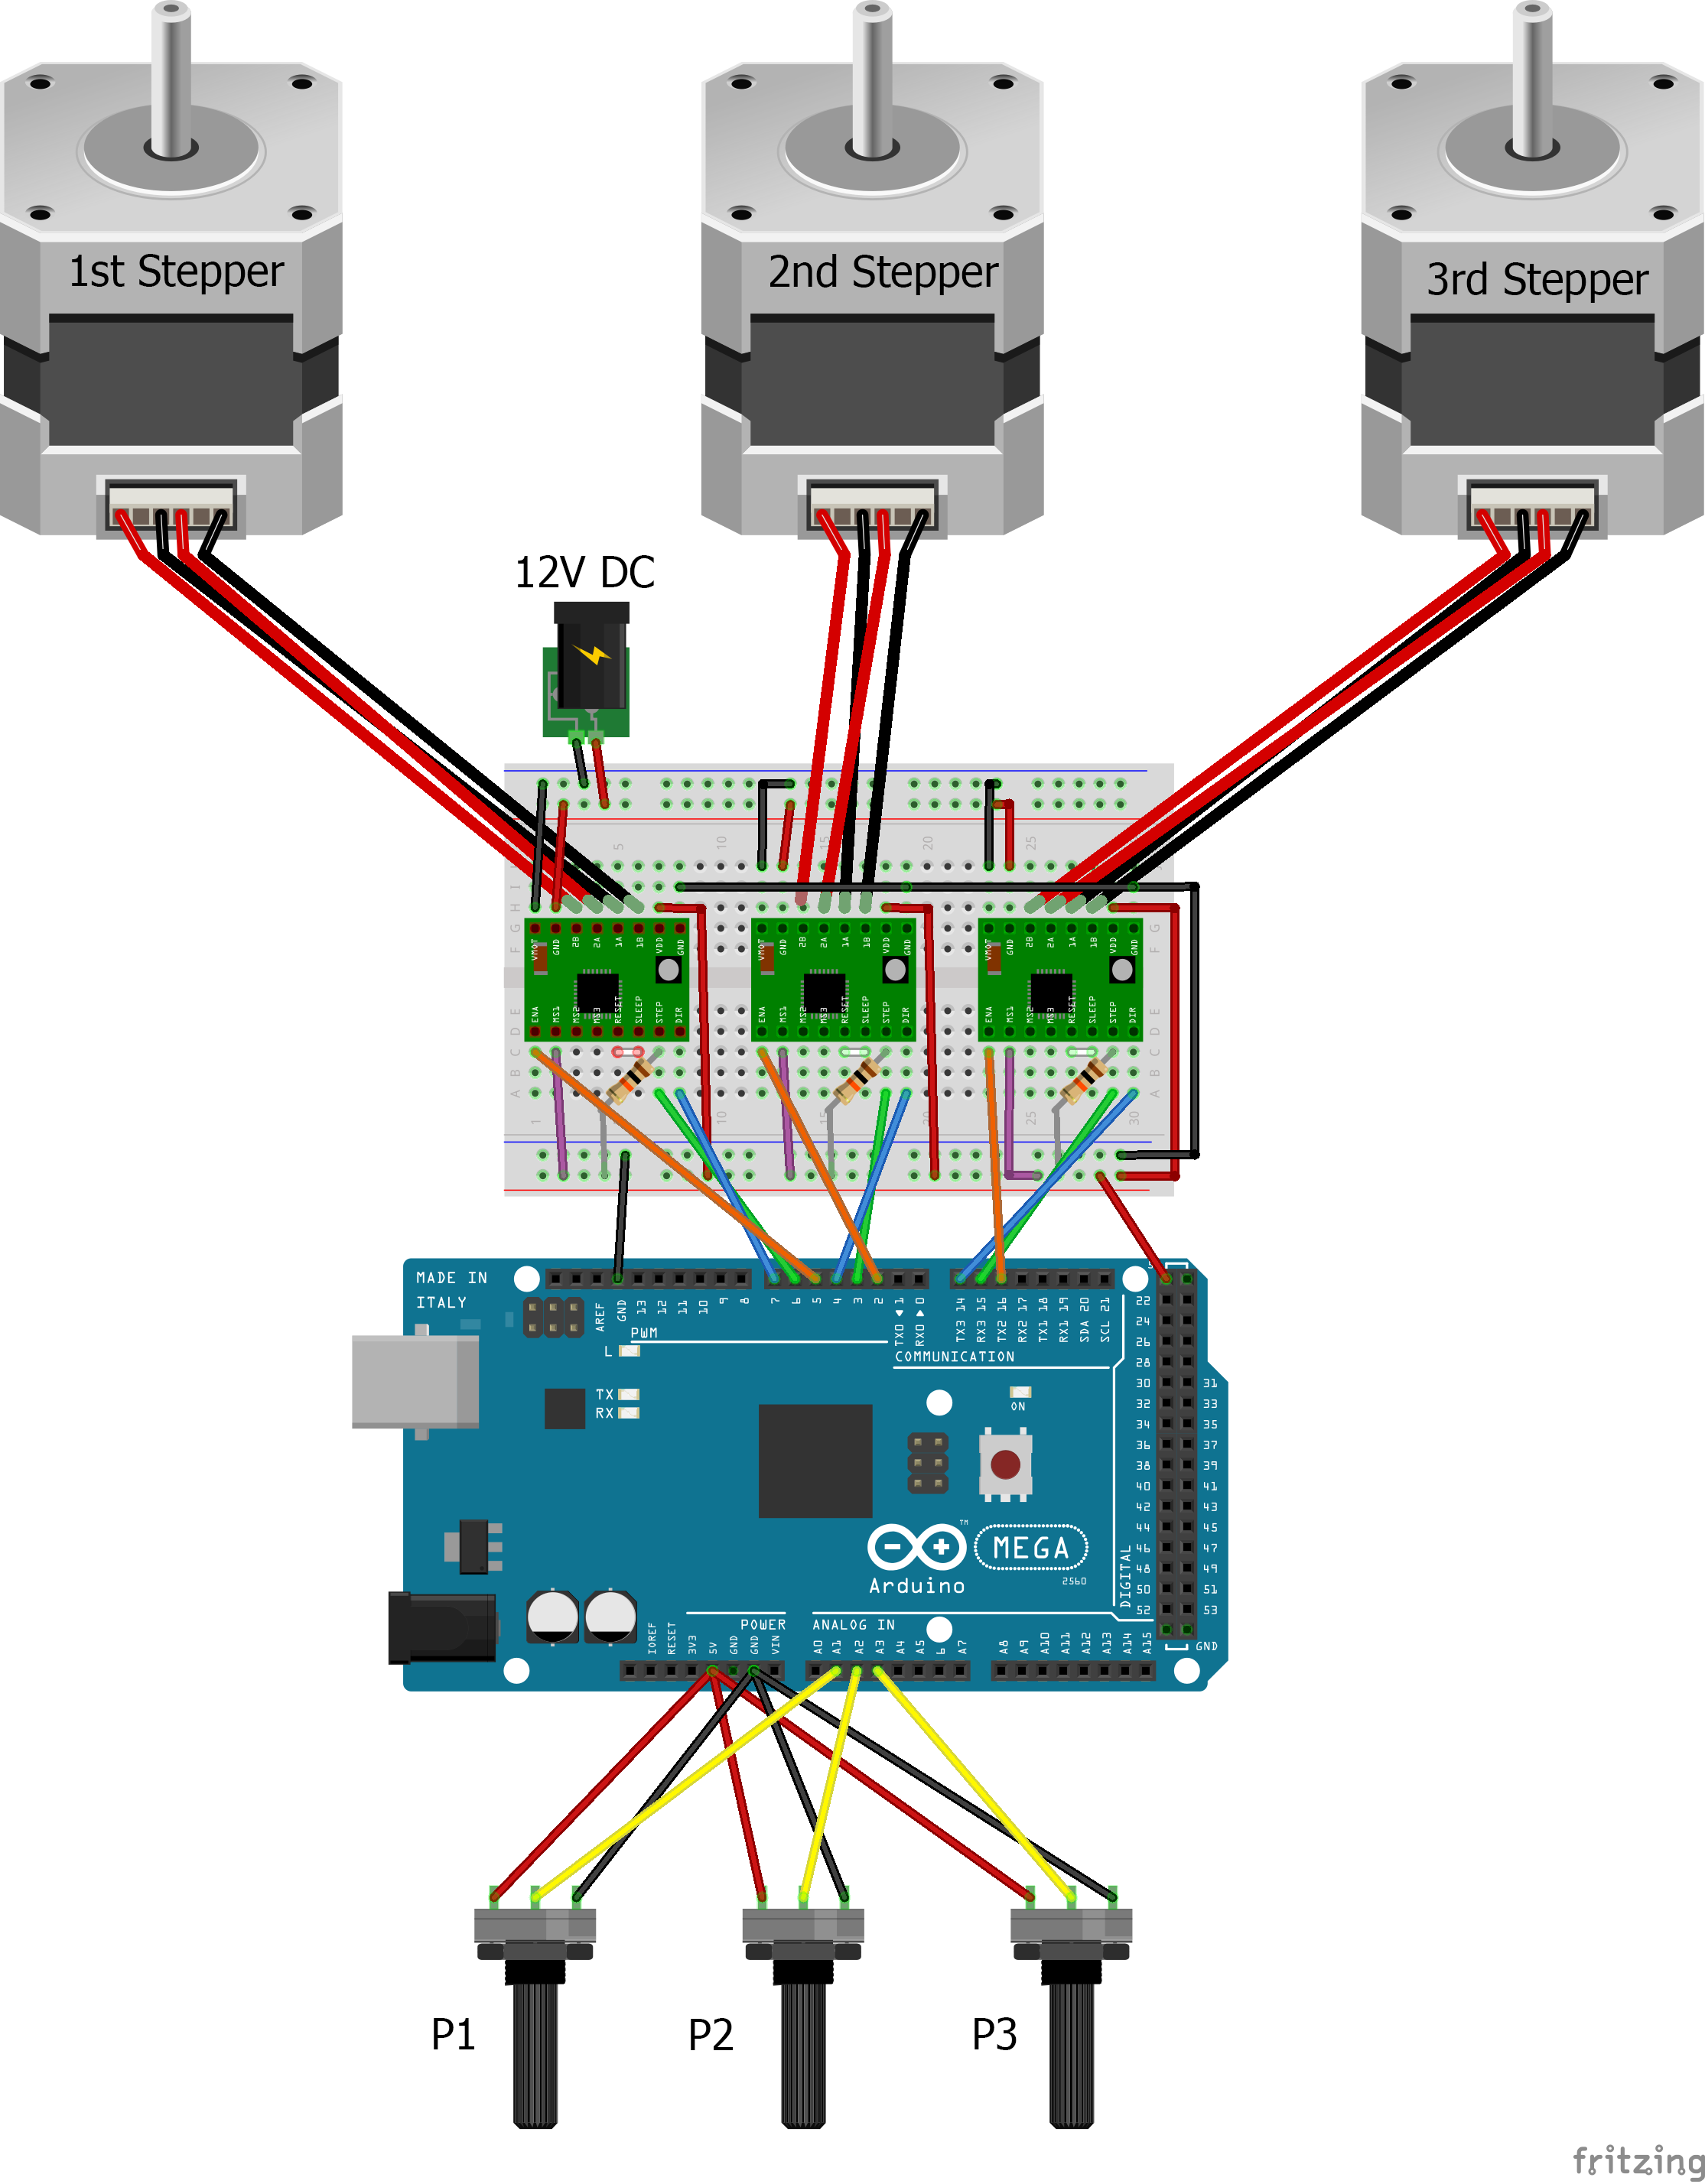
\includegraphics[width=\maxwidth{15cm}, keepaspectratio]{Chapters/Fig/stepper_coltroler_circuit.png}
	\caption{Stepper motor controller circuit}
	\label{fig:stepper_coltroler_circuit}
\end{figure}

\begin{figure}[H]
	\centering
	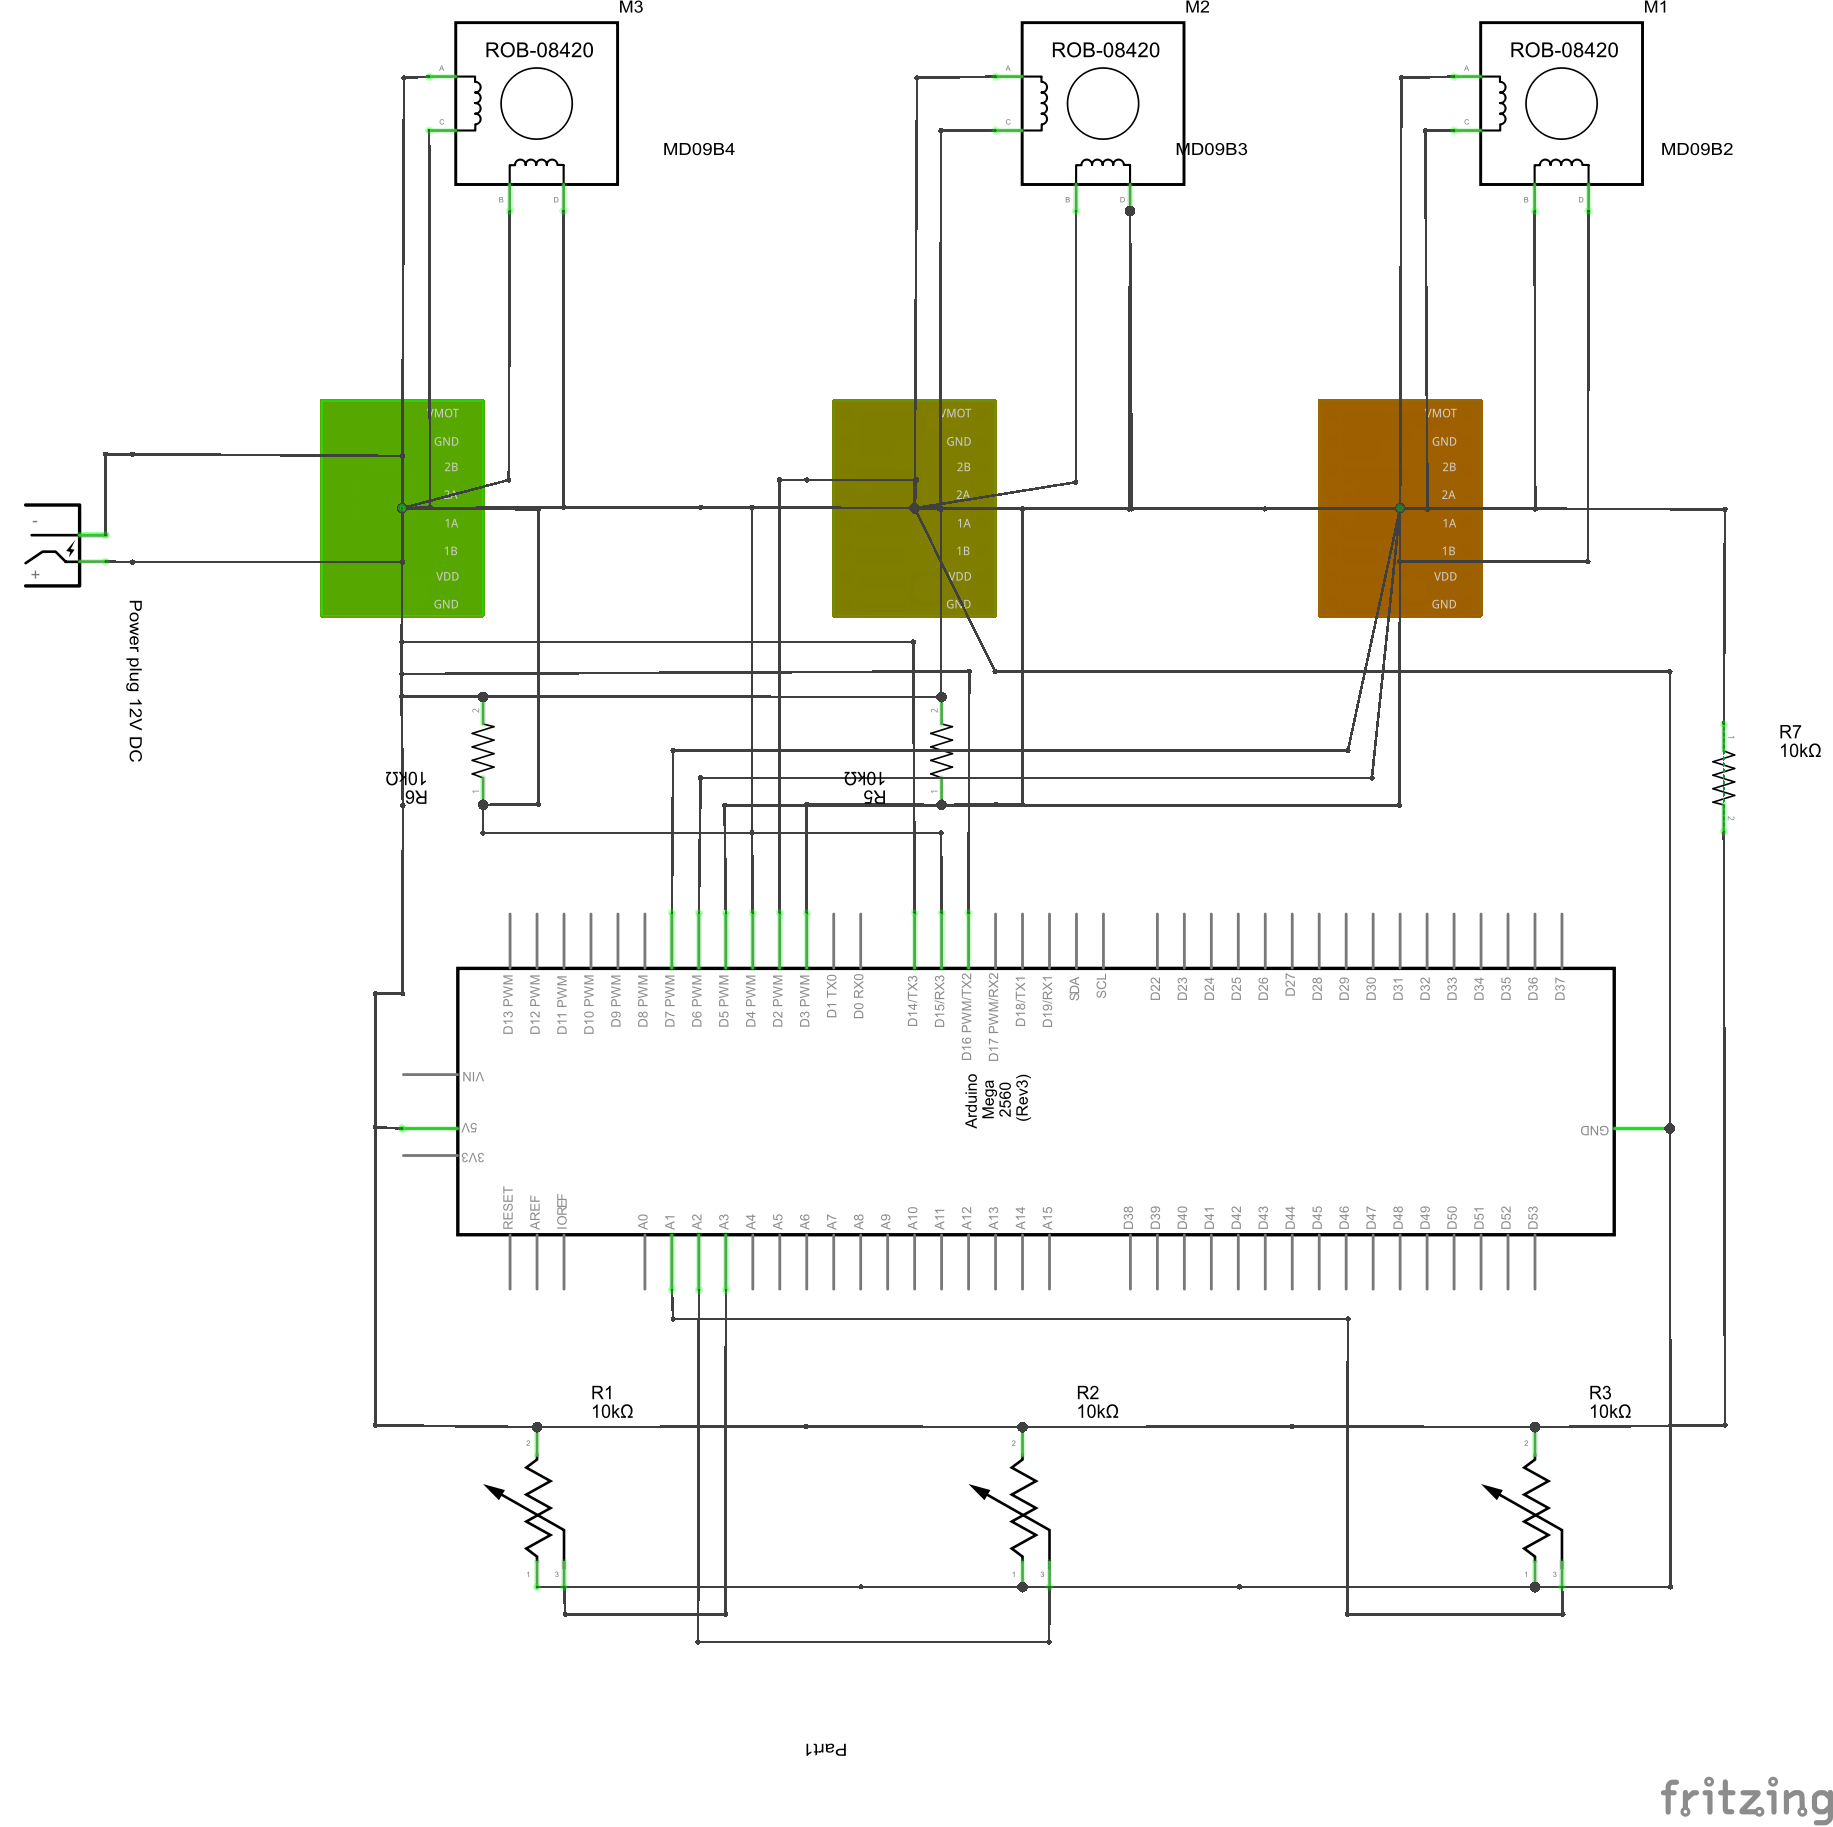
\includegraphics[width=\maxwidth{15cm}, keepaspectratio]{Chapters/Fig/stepper_coltroler_circuit_schem.png}
	\caption{Circuit diagram of stepper motor controller}
	\label{fig:stepper_coltroler_circuit_schem}
\end{figure}

\subsubsection{Digital Filtering}
Frequency interference is occured when the Robot is waiting for commands from server. The reason is that the input pin of the A4988 driver fell into undefined state (neirther 1 nor 0), then it's very susceptible to be interfer by the other frequencies. Specifically, in this case, it is interfer by 50 Hz frequency of the power supply.

To eliminate these interferences, we connect the STEP pin of A4988 driver to Vcc(+5V) by 10K Ohm resistor. 
As a consequence, the STEP pin of will be pushed in to HIGH voltage level instead of falling into undefined stage. This resolves the phenomenon of interference.

%Hiện tượng nhiễu tần số xảy ra khi Robot ở trong trạng thái chờ lệnh gửi đến từ server. Nguyên nhân là chân input của Arduino ở trạng thái ko xác định(không phải 1 cũng ko phải 0), khi đó nó rất dễ bị nhiễu bởi 1 tần số khác. cụ thể ở đây là tần số 50Hz của nguồn điện.
%Dể khử nhiễu chúng tôi đã dùng 1 điện trở 10K ohm để nối chân STEP của driver A4988 vs Vcc +5V. Lúc đó, thay vì chân STEP rơi vào trạng thái ko xác định, nó đc đẩy lên mức điện áp cao. Theo cách này hiện tượng nhiễu đã được giải quyết.

\subsection{LCD Displays circuit design}

Here are the pinouts from the LCD and the corresponding pin connection on the Arduino MEGA 2560:
\begin{table}[H]
	\centering
	\caption{Pinouts from the LCD and the corresponding pin connection on the Arduino}	
	\label{tab:LCD_connectto_Arduino}
	\begin{tabularx}{0.65\textwidth}{lll}
		\toprule
		\textbf{Symbol} & \textbf{Function} & \textbf{Arduino Pin} 	\\
		\midrule
		Vss & ground(0 V) & ground (0 V) 							\\
		\midrule
		Vdd & power (4.5 – 5.5 V) & +5V 							\\
		\midrule
		Vo & contrast adjustment & wiper( output) 					\\
		& & of 10k ohm potentiometer 								\\
		\midrule
		RS & H/L register select signal & 42 						\\
		\midrule
		R/W	& H/L read/write signal & ground (0 V) 					\\
		\midrule
		E & H/L enable signal	& 44 								\\
		\midrule
		DB4	& H/L data bus for 4-bit mode & 46 						\\
		\midrule
		DB5	& H/L data bus for 4--bit mode & 48 					\\
		\midrule
		DB6	& H/L data bus for 4-bit mode & 50 						\\
		\midrule
		DB7	& H/L data bus for 4-bit mode & 52 						\\
		\bottomrule
	\end{tabularx}
\end{table}

\begin{figure}[H]
	\centering
	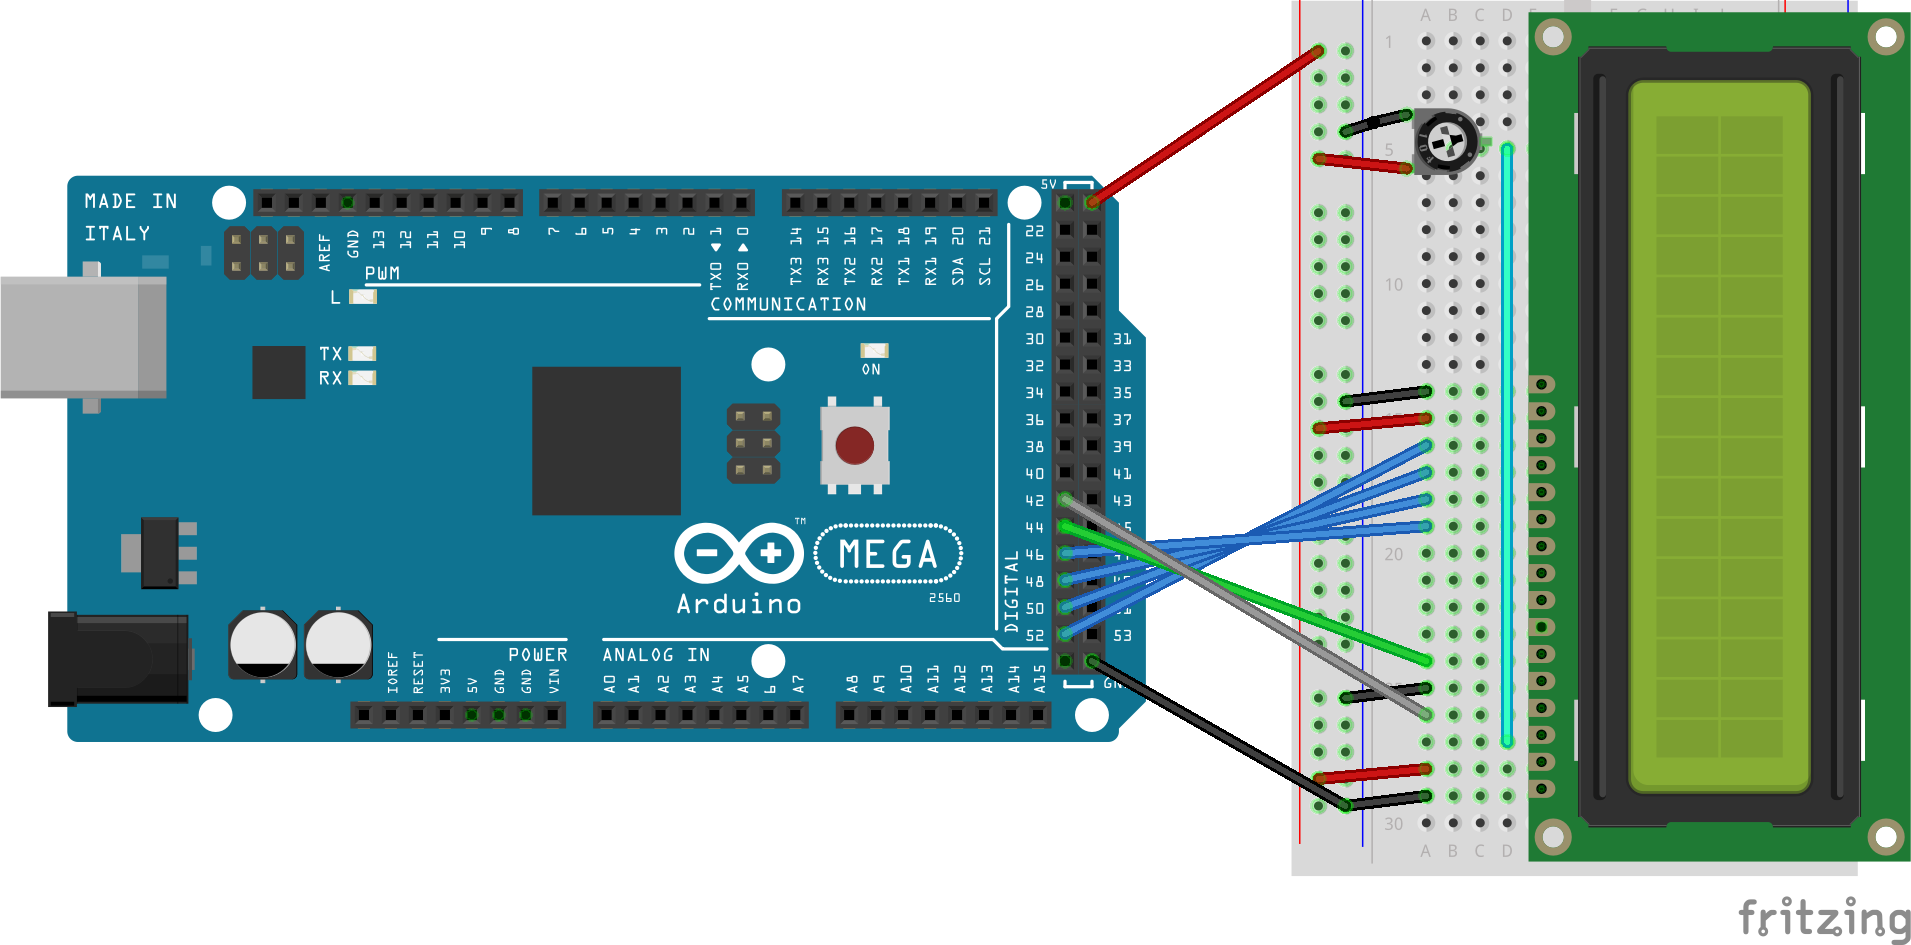
\includegraphics[width=\maxwidth{15cm}, keepaspectratio]{Chapters/Fig/deltarobot_LCD_16x2.png}
	\caption{LCD display interconnection}
	\label{fig:deltarobot_LCD_16x2}
\end{figure}

\begin{figure}[H]
	\centering
	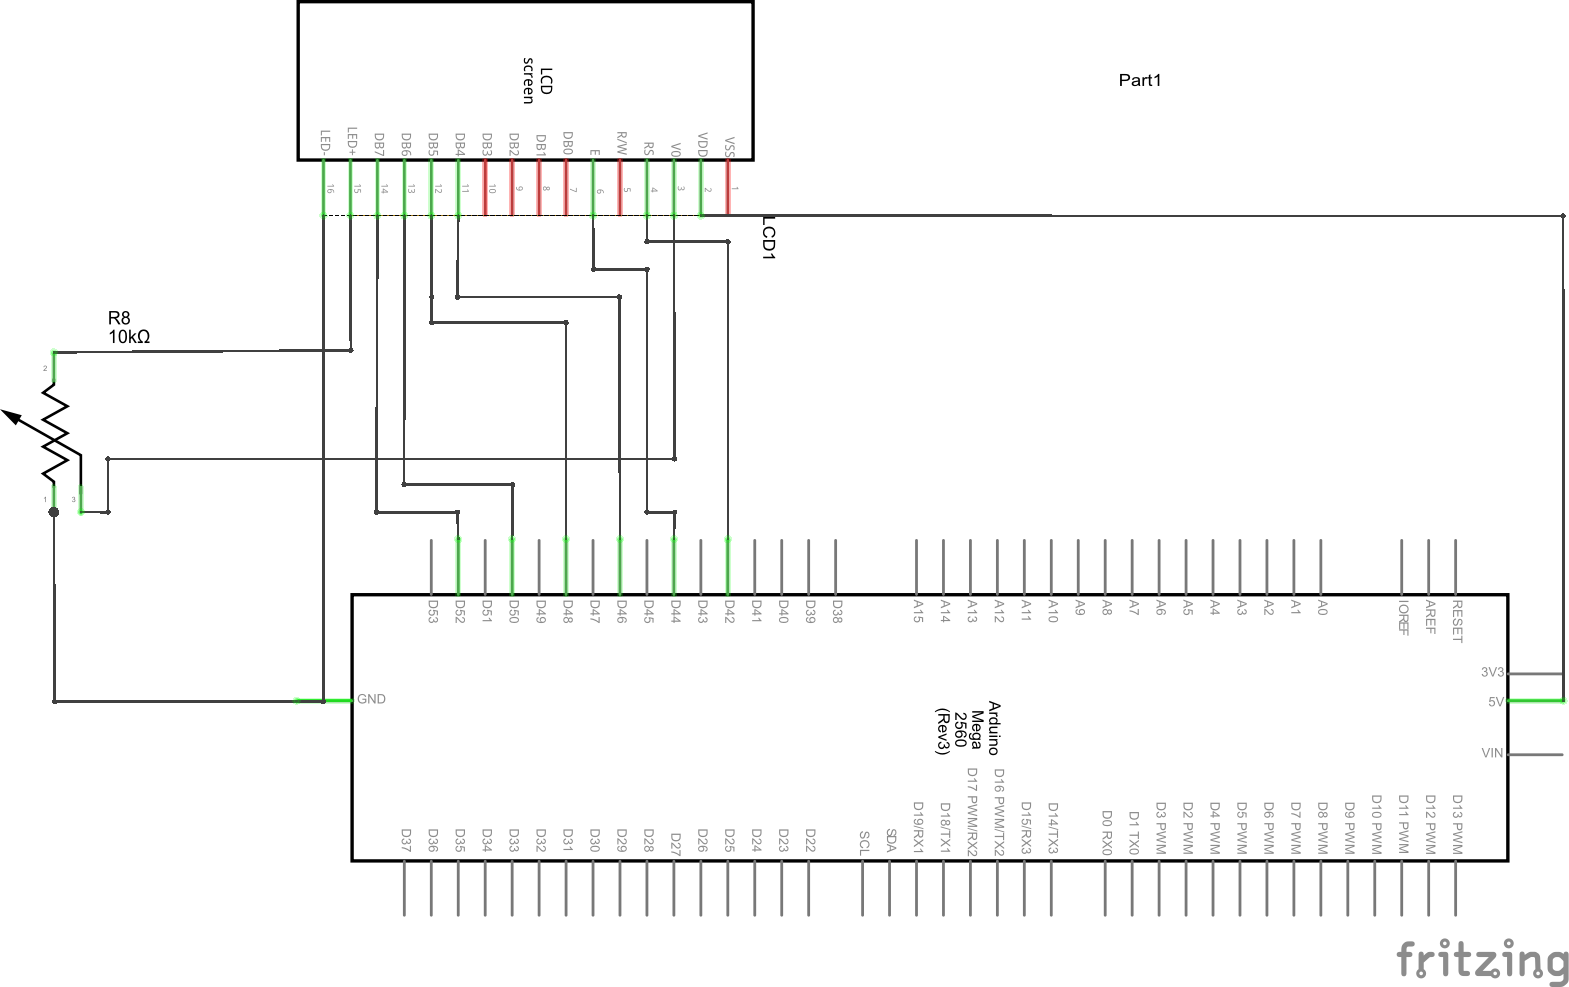
\includegraphics[width=\maxwidth{15cm}, keepaspectratio]{Chapters/Fig/Deltarobot_LCD_16x2_schem.png}
	\caption{Schematic of LCD Displays controller}
	\label{fig:Deltarobot_LCD_16x2_schem}
\end{figure}
\section{Software Design}

\subsection{Use cases diagram}
\subsubsection{Inverse kinematics}
\textbf{Actor:} User \\
\textbf{Summary:} User set coordinate of Delta robot's arms. C\# server necessary  to determine corresponding angles of three arms(joint angles)  and sent to Arduino microcontroller through USB connection. Arduino microcontroller drives three stepper motors to the received angle.
\begin{figure}[H]
	\centering
	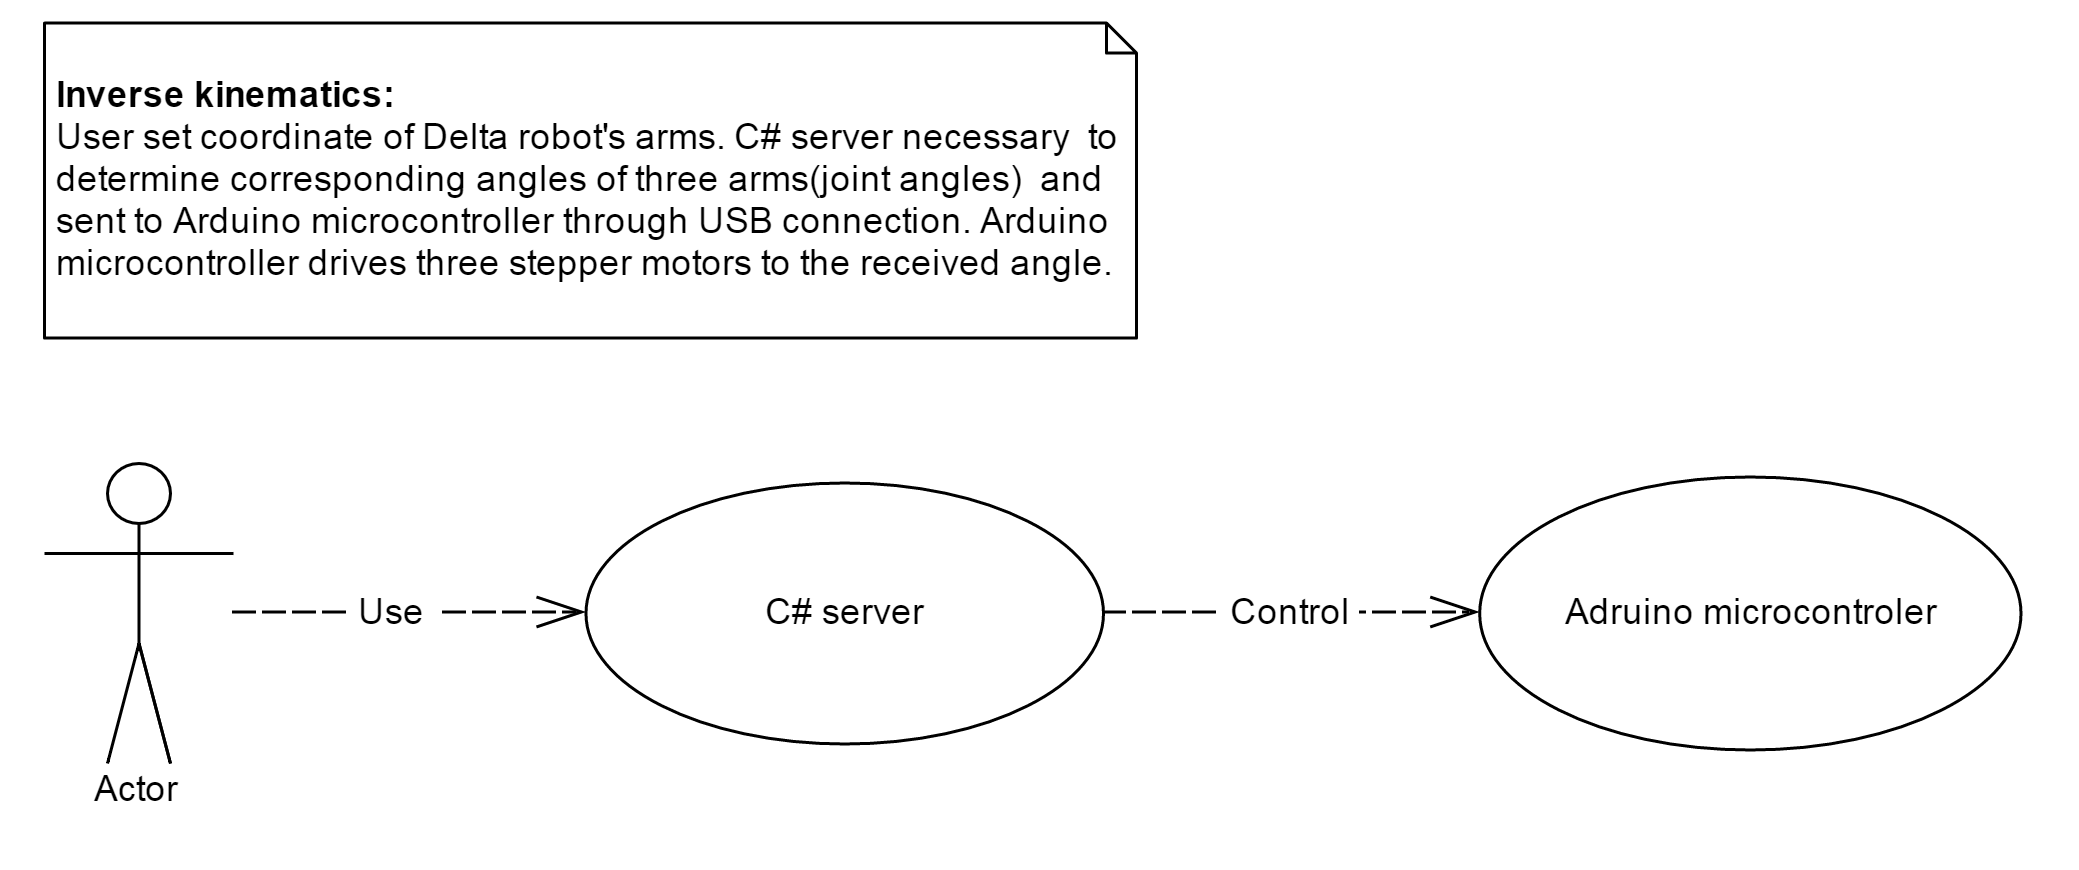
\includegraphics[width=\maxwidth{15cm}, keepaspectratio]{Chapters/Fig/usecase_inverse_kinematics.png}
	\caption{Inverse kinematics use cases diagram}
	\label{fig:usecase_inverse_kinematics}
\end{figure}

\subsubsection{Forward kinematics}
\textbf{Actor:} User \\
\textbf{Summary:} determine the possition of the end effector when the joint angles are known  
(i.e to make some corrections regarding its current possition)
\begin{figure}[H]
	\centering
	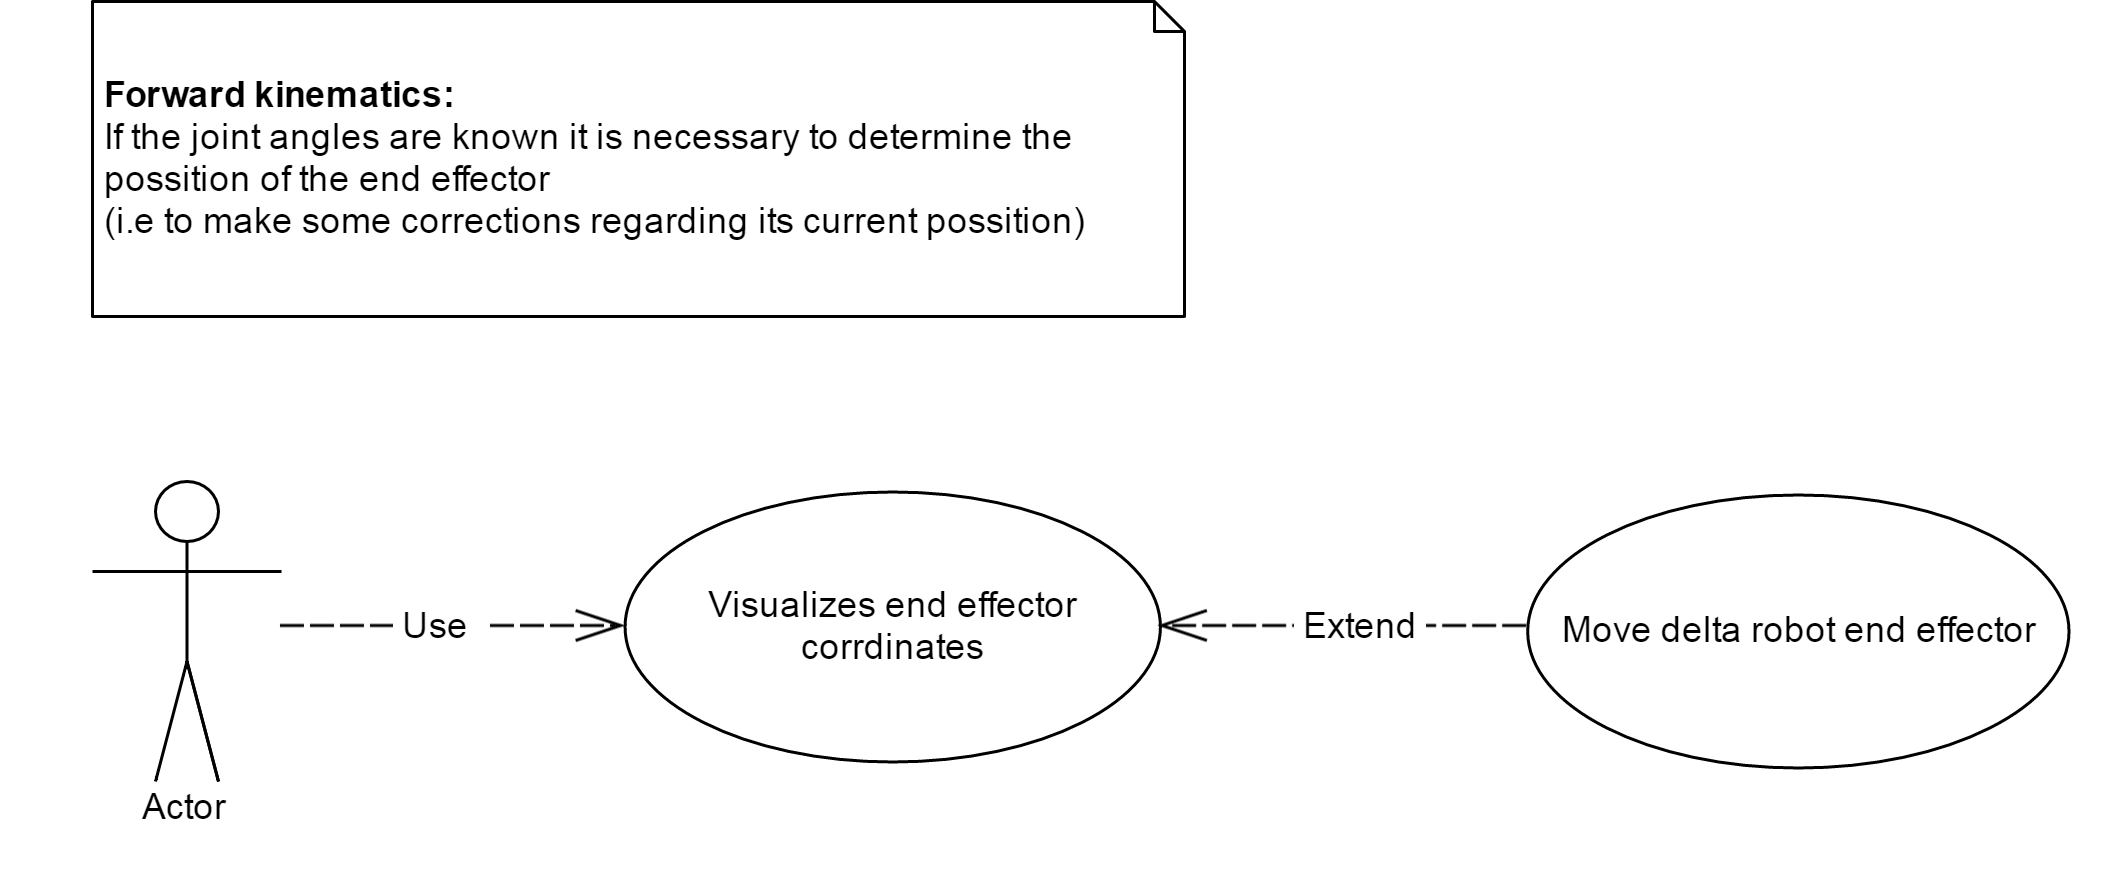
\includegraphics[width=\maxwidth{15cm}, keepaspectratio]{Chapters/Fig/usecase_forward_kinematics.png}
	\caption{Forward kinematics use cases diagram}
	\label{fig:usecase_forward_kinematics}
\end{figure}

\subsection{Class diagram}

\begin{figure}[H]
	\centering
	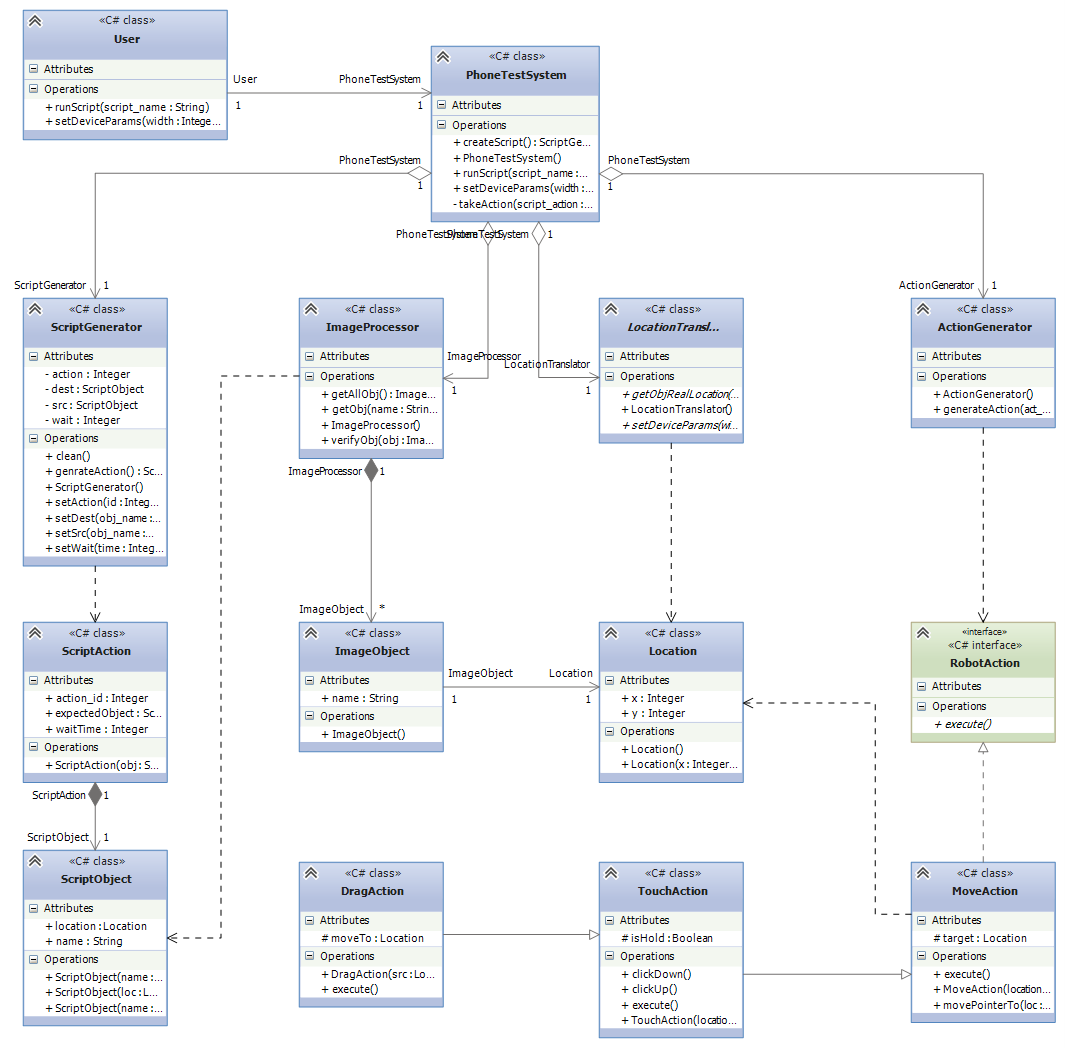
\includegraphics[width=\maxwidth{15cm}, keepaspectratio]{Chapters/Fig/class_diagram.png}
	\caption{Class diagram}
	\label{fig:class_diagram}
\end{figure}

When an action's execute method is invoked, it sends a moving command to Robot Controller. Robot Controller works like a black box. What outside clients see are high-level abstract methods. These methods include:

	\begin{itemize}
		\item[--] \textbf{InitPort}: initiate the connection with Arduino microcontroller.
		\item[--] \textbf{ClosePort}: destroy the connection with Arduino mcrocontroller.
		\item[--] \textbf{DetectArduino}: to check the connection.
		\item[--] \textbf{Calibrate}: set the robot's pointer to initial location which is supposed to be the origin point in coordination system.
		\item[--] \textbf{GotoXYZ}: most basic function, drive the pointer to any location in 3-D space.
		\item[--] \textbf{ClickUp}, \textbf{ClickDown}: also derived from GotoXYZ, simply make the pointer up or down correspondingly.
	\end{itemize}

Without assembly intervention to the robot, the system can still interact and dictate the robot fluently under the control of a singleton class Robot Controller. By applying ``Singleton Pattern'' \footnote{Read more at: \url{http://www.oodesign.com/singleton-pattern.html}}, the robot's activities is well-handled in a form of queue and thus avoid the interference of simultaneous commands.

\subsection{Sequence diagram}
\subsubsection{Inverse kinematics}
\begin{figure}[H]
	\centering
	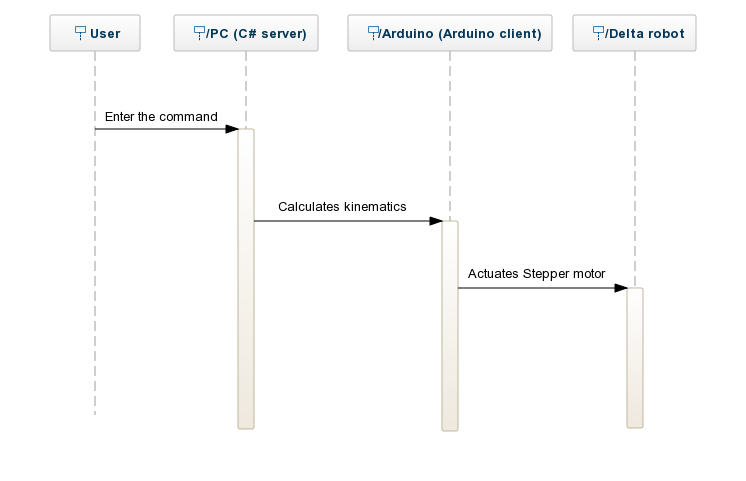
\includegraphics[width=\maxwidth{15cm}, keepaspectratio]{Chapters/Fig/inverse_kinematics_sequence_diagram.png}
	\caption{Sequence diagram of inverse kinematics}
	\label{fig:inverse_kinematics_sequence_diagram}
\end{figure}

\subsubsection{Forward kinematics}
\begin{figure}[H]
	\centering
	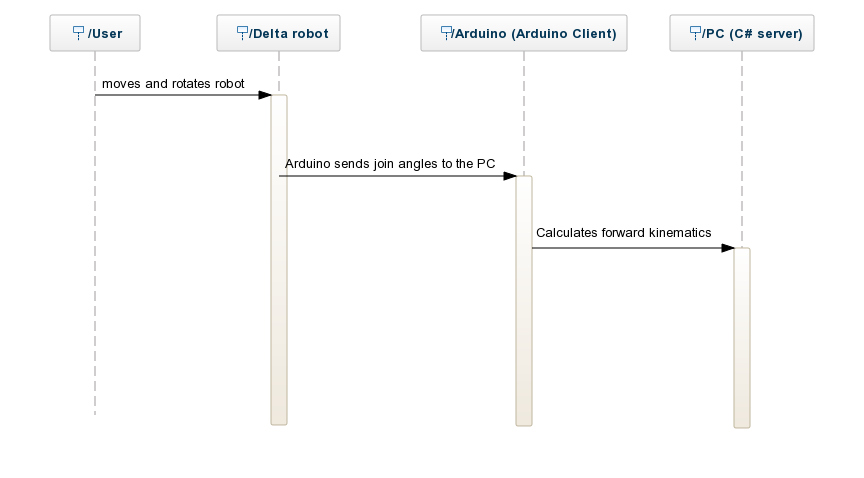
\includegraphics[width=\maxwidth{15cm}, keepaspectratio]{Chapters/Fig/forward_kinematics_sequence_diagram.png}
	\caption{Sequence diagram of forward kinematics}
	\label{fig:forward_kinematics_sequence_diagram}
\end{figure}

\subsection{Communications of CSharp and Arduino microcontroler via Serial Connection}

The C\# class combined with the Arduino sketch allows you to plug an Arduino into a PC's USB port and then have its COM port detected by the C\# application. Once the COM port is known the C\# application can then send/receive messages from the Arduino.

The concept is quite simple. The C\# application polls all the COM ports and sends a query using a simple protocol (explained below). Once the Arduino receives the request it replies. The C\# application that notes the COM port that caused the Arduino to reply and saves the name of the COM port. The C\# application can then use this COM port in subsequent communications.

\subsubsection{Communications Protocol}

To send a message I have to send 12 sets of bytes:

\begin{itemize}
		\item \textbf{Byte 0} is the start of command marker. This is always decimal 16 converted to byte (Convert.ToByte(16);)
		\item \textbf{Byte 1} is the type of command: 
		\begin{itemize}
		\item [ ] 128 = Identify
		\item [ ] 127 = Send data to pins
		\item [ ] 129 = Get data from arduino
		\item [ ] 130 = Set data to stepper motor
		\item [ ] 131 = Calibrate
		\end{itemize}
		\item \textbf{Byte 2} direction of 1st stepper
		\begin{itemize}
		\item [ ] 0 = DOWN
		\item [ ] 1 = UP
		\end{itemize}
		\item \textbf{Byte 3, Byte 4} is the number of steps of 1st stepper
		\begin{itemize}
		\item [ ] Byte 3 = numSteps / 256
		\item [ ] Byte 4 = numSteps \% 256
		\item [ ] (Number of steps between 0 to 65535)
		\end{itemize}
		\item \textbf{Byte 5} direction of 2nd stepper
		\begin{itemize}
		\item [ ] 0 = DOWN
		\item [ ] 1 = UP
		\end{itemize}
		\item \textbf{Byte 6, Byte 7} is the number of steps of 2nd stepper
		\begin{itemize}
		\item [ ] Byte 6 = numSteps / 256
		\item [ ] Byte 7 = numSteps \% 256
		\item [ ] (Number of steps between 0 to 65535)
		\end{itemize}
		\item \textbf{Byte 8} direction of 3rd stepper
		\begin{itemize}
		\item [ ] 0 = DOWN
		\item [ ] 1 = UP
		\end{itemize}
		\item \textbf{Byte 9, Byte 10} is the number of steps of 3rd stepper
		\begin{itemize}
		\item [ ] Byte 9 = numSteps / 256
		\item [ ] Byte 10 = numSteps \% 256
		\item [ ] (Number of steps between 0 to 65535)
		\end{itemize}
		\item \textbf{Byte 11} was used as an "end of message" marker but is redundant
\end{itemize}

\subsection{Control the Steppers}

How to move Delta robot's arm in a straight line?

The algorithm works by simple linear interpolation between two points given in 3-D space. It also adds in a linear acceleration and deceleration zone, near the endpoints.
In a nutshell, the manipulator moves a small increment forward along the path. Through inverse kinematics, I obtain a set of new arm angles. Given the current angles of the arm, I then calculate the number of stepper steps it will take for all the arms to reach the new angles. The steps then are distributed for all of the arms so that they all finish at the same time, providing a good enough approximation for straight line travel.

Example: Robot's arm needs to move from ($x_{0}$, $y_{0}$, $z_{0}$) to ($x_{1}$, $y_{1}$, $z_{1}$). Through inverse kinematics, I get a set of current and new arm angles are ($\theta1_{0}$, $\theta2_{0}$, $\theta3_{0}$) and ($\theta1_{1}$, $\theta2_{1}$, $\theta3_{1}$).
Speed and acceleration will be calculated by the math as follows:
\begin{flalign*}
& d_{\theta1} = \theta1_{1} - \theta1_{0} & \\
& d_{\theta2} = \theta2_{1} - \theta2_{0} & \\
& d_{\theta3} = \theta3_{1} - \theta3_{0} & \\
\end{flalign*}
$n_{1}$, $n_{2}$, $n_{3}$ in turn are the number of steps of stepper motor
\begin{flalign*}
& n_{1} = d_{\theta1} / STEP\_SIZE &\\
& n_{2} = d_{\theta2} / STEP\_SIZE &\\
& n_{3} = d_{\theta3} / STEP\_SIZE &\\
\end{flalign*}
$n_{MAX}$ is the largest step that stepper must execute. \\
$speed_{i} = n_{i} * MAX\_SPEED / n_{MAX}$; \\
$acceleration_{i} = n_{i} * MAX\_ACCELERATION / n_{MAX}$; \\





